\section{Introdução}

Alto-falantes são dispositivos eletromecânicos que convertem sinais elétricos em ondas sonoras, envolvendo fenômenos elétricos, magnéticos, mecânicos e acústicos. Seu comportamento pode ser representado por um conjunto de equações diferenciais que relacionam a corrente na bobina ao movimento do cone. 

Neste trabalho, é analisado inicialmente um modelo linear do alto-falante nos domínios do tempo e da frequência. Em seguida, é introduzida uma não linearidade no fator de força \(Bl\), permitindo comparar os modelos linear e não linear e avaliar os efeitos dessa alteração sobre a resposta do sistema. 

\section{Atividade 01 - Explorando o modelo linear}
\subsection{Sinal de entrada}

Para a análise do modelo linear, foi utilizado um sinal de áudio com duração de aproximadamente \(9\) segundos e taxa de amostragem de \(44100 \) Hz. O sinal foi normalizado de modo que sua amplitude permanecesse inferior a \(2\,V\), conforme especificado no enunciado.

\section{ Resultados da Atividade 1: resposta temporal e faixa estável de $\epsilon$.}

Na primeira etapa, analisou-se o comportamento do sistema em malha fechada para uma pequena perturbação na posição inicial, conforme proposto no enunciado. Para isso, foi considerada a condição inicial
  \[
  x(0) = x_0 + \epsilon,
  \]
  com
  \[
  \epsilon = 0{,}02x_0,
  \]

o que corresponde a uma perturbação de $2\%$ em relação à posição de
equilíbrio.

Os resultados obtidos indicam que o controlador PID foi capaz de estabilizar o sistema para essa condição inicial. A evidência principal disso está na resposta temporal da posição e da velocidade da peça. Observa-se que a posição retorna à vizinhança de $x_0$ ao longo do tempo, enquanto a velocidade tende a zero, caracterizando a convergência do sistema para um estado estável.

  \begin{figure}[H]
      \centering
       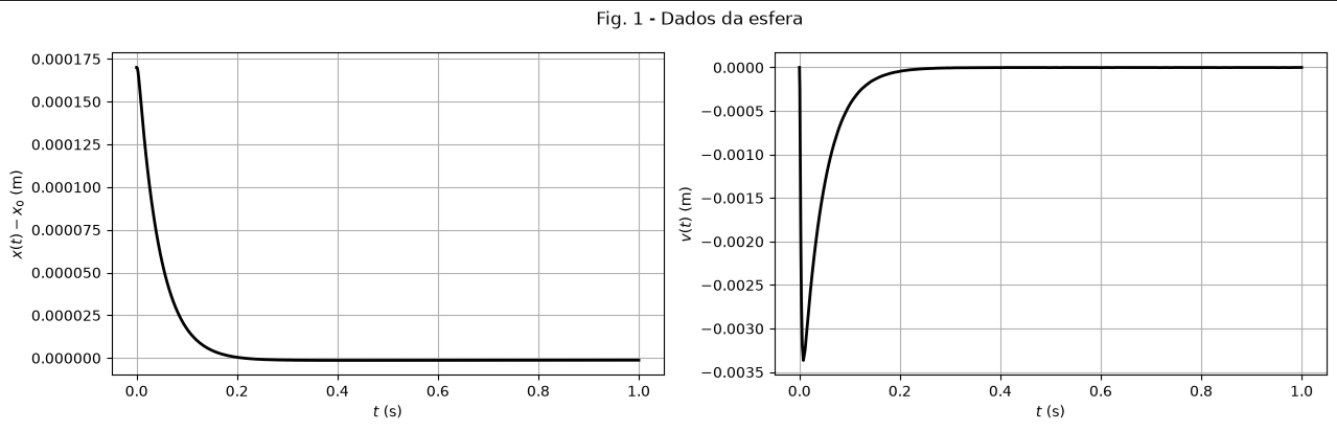
\includegraphics[width=0.9\textwidth]{imagens/grafico_posicao_velocidade.png}
      \caption{Resposta temporal da posição e da velocidade da peça para uma
      perturbação inicial de $2\%$ em relação a $x_0$.}
      \label{fig:posicao_velocidade_atividade1}
  \end{figure}

A Figura~\ref{fig:posicao_velocidade_atividade1} mostra que, após o deslocamento inicial, a peça não se afasta indefinidamente da posição de referência nem apresenta crescimento oscilatório. Pelo contrário, a trajetória permanece limitada e evolui em direção ao ponto de equilíbrio. Esse comportamento confirma que a ação de controle foi suficiente para compensar o efeito da perturbação inicial.

Do ponto de vista físico, isso significa que o controlador ajusta a tensão aplicada à bobina de modo a modificar a corrente elétrica e, consequentemente, a força magnética atuante sobre a peça. Esse mecanismo permite corrigir o desvio de posição e restabelecer o equilíbrio dinâmico do sistema.

Além da posição e da velocidade, a corrente elétrica também constitui uma evidência importante da atuação do controlador, pois representa diretamente o esforço de controle necessário para estabilizar o sistema. A análise desse sinal permite verificar se a correção exigida da fonte permanece dentro do limite admissível de operação.

  % Inserir aqui o gráfico da corrente
  \begin{figure}[H]
      \centering
       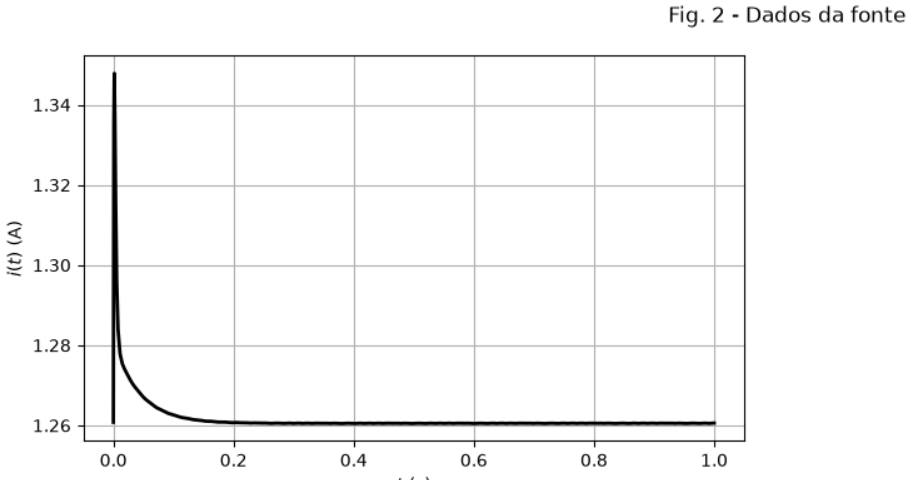
\includegraphics[width=0.75\textwidth]{imagens/grafico_corrente.png}
      \caption{Evolução temporal da corrente elétrica durante a estabilização do
      sistema para $\epsilon = 2\%$.}
      \label{fig:corrente_atividade1}
  \end{figure}

Os gráficos apresentados nas Figuras~\ref{fig:posicao_velocidade_atividade1} e~\ref{fig:corrente_atividade1} mostram que o controlador PID foi capaz de estabilizar o sistema para uma perturbação inicial de $2\%$. Observa-se que a posição retorna à vizinhança de $x_0$, enquanto a velocidade tende a zero ao longo do tempo, sem indicação de comportamento divergente. Além disso, a corrente permanece dentro do limite máximo de $2\,\text{A}$, mostrando que a estabilização ocorre de forma compatível com a restrição imposta à fonte.

Entretanto, esse resultado ainda corresponde a um caso particular. Para avaliar a faixa de perturbações iniciais para as quais o sistema permanece estável, foi realizada uma varredura numérica dos valores de $\epsilon$, sempre verificando também a restrição de corrente máxima. A partir dessa análise, obteve-se
\[
\epsilon_{\max} \approx 0{,}001165\ \text{m},
\]
o que corresponde a aproximadamente $13{,}71\%$ da posição de equilíbrio $x_0$.

\section{Resultados da Atividade 2: efeito do ruído na malha de realimentação}

  Na Atividade 2, foi introduzido ruído na medição da posição da peça, com média
  zero e desvio padrão dado por
  \[
  sd = 0{,}04x_0.
  \]

Com isso, o controlador PID passa a atuar sobre sinais medidos com incerteza, o que torna a malha mais sensível e dificulta a estabilização do sistema, principalmente devido ao termo derivativo.

  \begin{figure}[H]
      \centering
       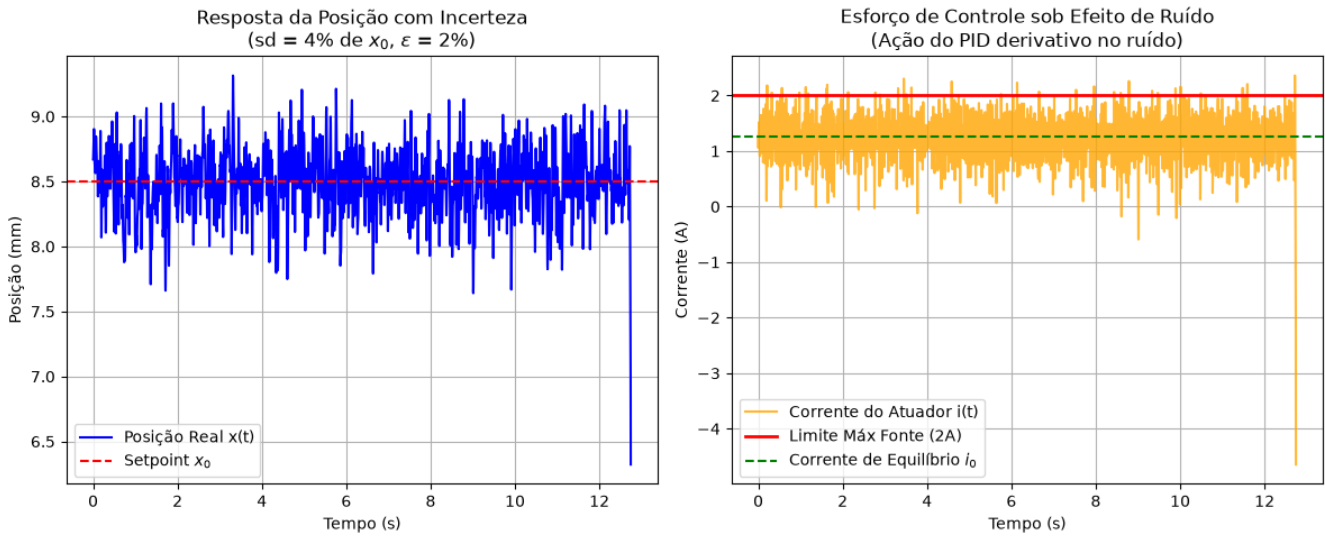
\includegraphics[width=0.9\textwidth]{imagens/grafico_ruido.png}
      \caption{Resposta do sistema com ruído na malha de realimentação.}
      \label{fig:ruido_atividade2}
  \end{figure}

A Figura~\ref{fig:ruido_atividade2} mostra que a presença de ruído prejudica o desempenho do controlador em comparação com o caso ideal. Além disso, a faixa de valores de $\epsilon$ para a qual o sistema permanece estável é reduzida, e o aumento de $sd$ torna a estabilidade ainda mais difícil de manter.

Assim, os resultados indicam que o controlador foi eficaz no caso ideal, mas se mostrou sensível à incerteza na medição.

\section{Conclusão}

Neste trabalho, foi possível modelar o sistema de levitação magnética em espaço de estados e aplicar um controlador PID para estabilizar a posição da peça em torno do ponto de equilíbrio. Na Atividade 1, os resultados mostraram que o controlador foi capaz de estabilizar o sistema para pequenas perturbações iniciais, mantendo também a corrente dentro do limite especificado.

Na Atividade 2, observou-se que a presença de ruído na malha de realimentação prejudica o desempenho do controlador e reduz a faixa de estabilidade do sistema. Assim, conclui-se que o PID adotado foi eficaz no caso ideal, mas apresenta sensibilidade à incerteza de medição.